%%%%%%%%%%%%%%%%%%%%%%%%%%%%%%%%%%%%%%%%%%%%%%%%%%%%%%%%%%%%%%%%%%%%%%%%%%%%%%%%
\chapter{Тестирование инструмента автоматизированной генерации спецификации}
%%%%%%%%%%%%%%%%%%%%%%%%%%%%%%%%%%%%%%%%%%%%%%%%%%%%%%%%%%%%%%%%%%%%%%%%%%%%%%%%

В этом разделе разработанный инструмент автоматизированной генерации спецификации проходит на проверку на то, чтобы все требования, которые были поставлены в начале работы, были соблюдены.

%%%%%%%%%%%%%%%%%%%%%%%%%%%%%%%%%%%%%%%%%%%%%%%%%%%%%%%%%%%%%%%%%%%%%%%%%%%%%%%%
\section{Тестирование}
%%%%%%%%%%%%%%%%%%%%%%%%%%%%%%%%%%%%%%%%%%%%%%%%%%%%%%%%%%%%%%%%%%%%%%%%%%%%%%%%

Главной задачей в данном разделе было показать примеры генерации спецификации на различных библиотеках, начиная с простой самописной вручную, заканчивая полноценной библиотекой.

%%%%%%%%%%%%%%%%%%%%%%%%%%%%%%%%%%%%%%%%%%%%%%%%%%%%%%%%%%%%%%%%%%%%%%%%%%%%%%%%
\subsection{Тестирование на простой библиотеке}
%%%%%%%%%%%%%%%%%%%%%%%%%%%%%%%%%%%%%%%%%%%%%%%%%%%%%%%%%%%%%%%%%%%%%%%%%%%%%%%%

В качестве простой библиотеки подразумевается небольшая самописная состоящая из нескольких простых классов и одного интерфейса

Результат работы инструмента с этой библиотекой является lsl файл, фрагмент которого приведен ниже:
\begin{figure}[htbp]
\centering
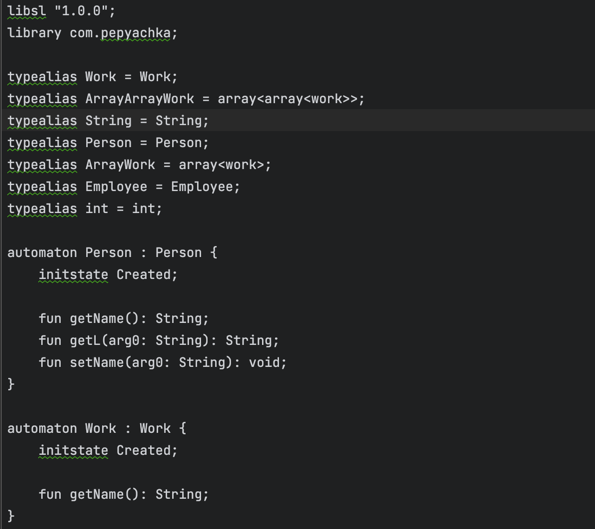
\includegraphics[width=\textwidth]{fig/my_libsl.png}
\caption{Пример сгенерированного LibSL}%
\label{fig:my_libsl}
\end{figure}

%%%%%%%%%%%%%%%%%%%%%%%%%%%%%%%%%%%%%%%%%%%%%%%%%%%%%%%%%%%%%%%%%%%%%%%%%%%%%%%%
\subsection{Тестирование на библиотеке okhttp3}
%%%%%%%%%%%%%%%%%%%%%%%%%%%%%%%%%%%%%%%%%%%%%%%%%%%%%%%%%%%%%%%%%%%%%%%%%%%%%%%%

Для еще одного этапа тестирования была выбрана библиотека okhttp3

Результат работы инструмента с этой библиотекой является lsl файл, фрагмент которого приведен ниже:
\begin{figure}[htbp]
\centering
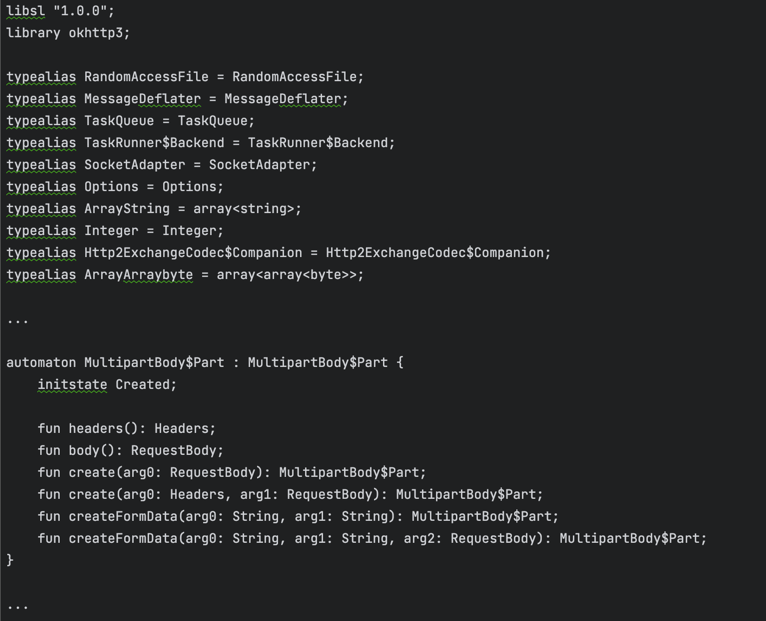
\includegraphics[width=\textwidth]{fig/okhttp_libsl.png}
\caption{Пример сгенерированного LibSL для библиотеки okhttp}%
\label{fig:okhttp_libsl}
\end{figure}

Для экономии места часть кода была удалена.

%%%%%%%%%%%%%%%%%%%%%%%%%%%%%%%%%%%%%%%%%%%%%%%%%%%%%%%%%%%%%%%%%%%%%%%%%%%%%%%%
\section{Тестирование результатов с помощью парсера}
%%%%%%%%%%%%%%%%%%%%%%%%%%%%%%%%%%%%%%%%%%%%%%%%%%%%%%%%%%%%%%%%%%%%%%%%%%%%%%%%

Единственным автоматизированным способом проверки разработанного инструмента является существующий парсер LibSL спецификации \cite{libsl_parser}.

Ниже представлен фрагмент кода, показывающий взаимодействие с данной библиотекой:
\lstinputlisting[
label={listings:javaparser},
caption={Валидация сгенерированного LibSL файла с помощью парсера},
style=java,
]
{src/fragments/LibSLParserExample.java}

На вход парсеру падается сгенерированный файл спецификации с расширением lsl. Парсер в свою очередь преобразует спецификацию в абстрактный семантический граф.
Если результатом является какое-либо исключение, нетрудно догадаться, что в спецификации есть ошибки, на которые парсер также явно указывает в выводе.

%%%%%%%%%%%%%%%%%%%%%%%%%%%%%%%%%%%%%%%%%%%%%%%%%%%%%%%%%%%%%%%%%%%%%%%%%%%%%%%%
\section{Вывод}
%%%%%%%%%%%%%%%%%%%%%%%%%%%%%%%%%%%%%%%%%%%%%%%%%%%%%%%%%%%%%%%%%%%%%%%%%%%%%%%%

В данном разделе была рассмотрена программа тестирования с помощью предложенного парсера LibSL спецификаций, а также данный раздел включает в себя фрагменты сгенерированных спецификаций на различных библиотеках.
Тестирование показало, что инструмент выполняет поставленные перед ним задачи генерации спецификации.

